\documentclass[aspectratio=169, 11pt]{beamer}
% \documentclass[aspectratio=169, 11pt, handout]{beamer}

% ── Theme ──
\usetheme{Madrid}
\usecolortheme{default}
\setbeamertemplate{navigation symbols}{}
\setbeamertemplate{footline}{%
  \leavevmode\hbox{%
    \begin{beamercolorbox}[wd=.333333\paperwidth,ht=2.5ex,dp=1ex,center]{author in head/foot}%
      \usebeamerfont{author in head/foot}\insertshortauthor
    \end{beamercolorbox}%
    \begin{beamercolorbox}[wd=.333333\paperwidth,ht=2.5ex,dp=1ex,center]{title in head/foot}%
      \usebeamerfont{title in head/foot}\insertshorttitle
    \end{beamercolorbox}%
    \begin{beamercolorbox}[wd=.333333\paperwidth,ht=2.5ex,dp=1ex,right]{date in head/foot}%
      \usebeamerfont{date in head/foot}\insertframenumber{} / \inserttotalframenumber\hspace*{2ex}
    \end{beamercolorbox}}}

% ── Packages ──
\usepackage{amsmath,amssymb}
\usepackage{booktabs}
\usepackage{xcolor}
\usepackage{colortbl}
\usepackage{tikz}
\usetikzlibrary{arrows.meta, positioning}
\usetikzlibrary{calc}

% ── Colors ──
\definecolor{sbgreen}{HTML}{00704A}
\definecolor{abnbred}{HTML}{FF5A5F}
\definecolor{warnred}{HTML}{CC0000}
\definecolor{noteblue}{HTML}{2060A0}

% ── Commands ──
\newcommand{\E}{\mathbb{E}}
\newcommand{\Var}{\mathrm{Var}}
\newcommand{\Cov}{\mathrm{Cov}}
\newcommand{\SE}{\mathrm{SE}}
\newcommand{\Prob}{\mathrm{Pr}}
\newcommand{\indep}{\perp\!\!\!\perp}
\DeclareMathOperator{\plim}{plim}

% ── Reusable TikZ styles ──
\tikzset{
    tnode/.style={draw, rounded corners, fill=gray!10, minimum width=2.2cm, minimum height=0.65cm, font=\small, align=center},
    tgreen/.style={tnode, fill=sbgreen!15, draw=sbgreen},
    tblue/.style={tnode, fill=noteblue!12, draw=noteblue},
    tred/.style={tnode, fill=abnbred!15, draw=abnbred},
    twarn/.style={tnode, fill=red!8, draw=warnred},
    tarrow/.style={-{Stealth}, thick}
}

% ── Title ──
\title[Lecture 7]{Lecture 7: When You Can't Randomize}
\subtitle{Applied ML for Business Part II}
\author{Zhikun Lu}
\date{\today}

\begin{document}

% ====================================================================
\begin{frame}
\titlepage
\end{frame}

% ====================================================================
\begin{frame}{Module 4 Roadmap}

\begin{center}
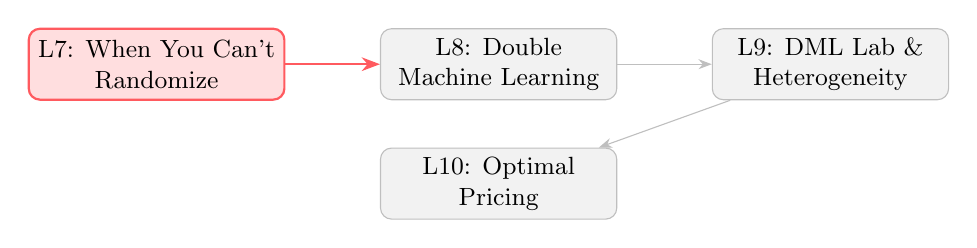
\begin{tikzpicture}[
    node distance=0.6cm and 1.2cm,
    box/.style={draw, rounded corners, minimum width=3cm, minimum height=0.9cm, font=\small, align=center},
    active/.style={box, fill=abnbred!20, draw=abnbred, thick},
    inactive/.style={box, fill=gray!10, draw=gray!50}
]
\node[active]                (L7)  {L7: When You Can't\\Randomize};
\node[inactive, right=of L7] (L8)  {L8: Double\\Machine Learning};
\node[inactive, right=of L8] (L9)  {L9: DML Lab \&\\Heterogeneity};
\node[inactive, below=of L8] (L10) {L10: Optimal\\Pricing};

\draw[-{Stealth}, thick, abnbred] (L7) -- (L8);
\draw[-{Stealth}, gray!50]        (L8) -- (L9);
\draw[-{Stealth}, gray!50]        (L9) -- (L10);
\end{tikzpicture}
\end{center}

\bigskip

\textbf{Module 3:} Binary treatment. Randomization gave us identification for free.

\smallskip

\textbf{Module 4:} Continuous treatment. No randomization. Identification requires assumptions, and those assumptions carry real content.

\end{frame}

% ====================================================================
\begin{frame}{Today's Plan}

\textbf{From Experiments to Observational Data}

\begin{enumerate}
    \item \textbf{The business problem.} Pricing suggestions: data, demand model, and naive estimates
    \item \textbf{The causal framework.} Potential outcomes, assumptions, and identification
    \item \textbf{The estimation gap.} Why traditional econometrics (OLS) and machine learning (Lasso) both fail; what we actually need
\end{enumerate}

\bigskip

\textbf{Next time (Lecture 8):} Double Machine Learning fills the gap.

\end{frame}


% %%%%%%%%%%%%%%%%%%%%%%%%%%%%%%%%%%%%%%%%%%%%%%%%%%%%%%%%%%%%%%%%%%%%
\section{The Problem}
% %%%%%%%%%%%%%%%%%%%%%%%%%%%%%%%%%%%%%%%%%%%%%%%%%%%%%%%%%%%%%%%%%%%%
\begin{frame}{The Business Problem}

\textbf{Airbnb} wants to build a Smart Pricing tool: suggest an optimal nightly rate to each host. 

\bigskip

\textbf{Data:} clearly a data-driven problem; for each listing, we observe 
\begin{itemize}
    \item the nightly price (P) and 
    \item the number of nights booked per month (Q).
\end{itemize}

\bigskip

\textbf{Goal:} to set the right price, we need to understand how price P \textbf{affects} demand Q\\
$\Longrightarrow$ this is a classical demand curve problem: $Q= f(P)$

\end{frame}


\begin{frame}{The Demand Model}

A key object is the slope $\Delta Q / \Delta P$. A unit-free version is the \textbf{price elasticity of demand}:
\[
\theta \equiv \frac{\partial \log Q}{\partial \log P} \approx \frac{\Delta Q / Q}{\Delta P / P}
\]

\textbf{Interpretation}: \textit{If a host raises their price by 1\%, the number of nights sold increases by $\theta$\%.}

\bigskip
\pause

\textbf{Why elasticity matters?} A profit-maximizing host solves $\max_P (P - c) \cdot f(P)$. The first-order condition gives the \textbf{inverse elasticity pricing rule}:
\[
\frac{P^* - c}{P^*} = -\frac{1}{\theta(P^*)}
\]

The optimal price $P^*$ depends only on the elasticity.

\end{frame}

\begin{frame}{The Demand Model}

In general, $\theta(P)$ depends on where $P$ is on the demand curve. 

\pause
\bigskip

Assuming constant elasticity $\theta$ gives the \textbf{isoelastic demand model}: $Q = A \cdot P^{\theta}$.

\begin{itemize}
    \item The optimal pricing rule is a constant markup over cost: 
    $$\mu = \frac{P}{c} = \frac{\theta}{\theta+1}$$
    \item Taking logs with $Y = \log Q$, $D = \log P$, $\alpha=\log(A)$ and adding a noise term:
    \[
    \Longrightarrow Y = \alpha + \theta \cdot D + \epsilon,
    \]
    \item This is something we can estimate using linear regression.
\end{itemize}

\end{frame}


% ====================================================================
\begin{frame}{Price Elasticity as a Causal Parameter}

The elasticity answers a \textbf{causal} question: what \emph{would happen} if a host changed their price?

\bigskip

This is not the same as comparing hosts who charge different prices. A listing at \$200/night may sell \emph{more} than one at \$100/night, because it is a nicer apartment.

\bigskip
\pause

Estimating $\theta$ requires \textbf{causal variation in prices}: variation not driven by listing quality. 

\bigskip

The most ideal source is \textbf{randomization}, but not always available.

\end{frame}


\begin{frame}{When We Can and Cannot Randomize}

Companies with pricing control (possible to experiment):
\begin{itemize}
    \item \textbf{Starbucks} (including coupons), \textbf{Amazon Retail} (sold by Amazon)
    \item \textbf{DiDi} or \textbf{Uber} (ride-hailing company) directly set prices for both passengers and drivers
    \item \textbf{Pinduoduo} (e-commerce platform) and \textbf{Temu} (PDD's oversea version) may force sellers to adjust prices, though this practice comes with potential legal concerns
\end{itemize}

\medskip

Companies without pricing control (no experiments):
\begin{itemize}
    \item \textbf{Airbnb}: Hosts set prices; the platform may \emph{suggest} but cannot \emph{assign} without consent
    \item \textbf{Amazon Marketplace}: Third-party sellers set prices; ``competitive pricing'' tools
    \item \textbf{Zillow}: Sellers/agents choose listing prices; ``Zestimate'' serves as a reference
\end{itemize}

\end{frame}



% ====================================================================
\begin{frame}{Observational Data}

Six listings: three entire apartments (type $A$) and three private rooms (type $B$).

\medskip

\begin{center}
\begin{tabular}{clcccc}
\toprule
\textbf{Listing} & \textbf{Type} & \textbf{Price} & \textbf{Log price $D$} & \textbf{Nights/mo} & \textbf{Log nights $Y$} \\
\midrule
1 & Entire apt ($A$) & \$90 & 4.5 & 33 & 3.5 \\
2 & Entire apt ($A$) & \$148 & 5.0 & 20 & 3.0 \\
3 & Entire apt ($A$) & \$245 & 5.5 & 12 & 2.5 \\
\midrule
4 & Private room ($B$) & \$20 & 3.0 & 3 & 1.0 \\
5 & Private room ($B$) & \$33 & 3.5 & 2 & 0.5 \\
6 & Private room ($B$) & \$55 & 4.0 & 1 & 0.0 \\
\bottomrule
\end{tabular}
\end{center}

% \medskip
% \pause

% The true DGP is $Y_i = \theta D_i + g(\text{type}_i) + \varepsilon_i$ with $\theta = -1$, $g(A) = 8$, $g(B) = 4$, $\varepsilon_i = 0$.

% \bigskip

% \textbf{Key pattern:} type $A$ has higher prices \emph{and} higher demand. This is $g(X)$ at work. Can a naive regression separate $\theta$ from $g$?

\end{frame}

% ====================================================================


% ====================================================================
\begin{frame}{The Naive Analysis}

With $\bar{D} = 4.25, \bar{Y} = 1.75$, we have

\begin{center}
\scriptsize
\begin{tabular}{clcccc}
\toprule
$i$ & Type & $D_i - \bar{D}$ & $Y_i - \bar{Y}$ & $(D_i-\bar{D})^2$ & $(D_i-\bar{D})(Y_i-\bar{Y})$ \\
\midrule
1 & $A$ & $+0.25$ & $+1.75$ & $0.0625$ & $+0.4375$ \\
2 & $A$ & $+0.75$ & $+1.25$ & $0.5625$ & $+0.9375$ \\
3 & $A$ & $+1.25$ & $+0.75$ & $1.5625$ & $+0.9375$ \\
4 & $B$ & $-1.25$ & $-0.75$ & $1.5625$ & $+0.9375$ \\
5 & $B$ & $-0.75$ & $-1.25$ & $0.5625$ & $+0.9375$ \\
6 & $B$ & $-0.25$ & $-1.75$ & $0.0625$ & $+0.4375$ \\
\midrule
  &   & & & $4.375$ & $4.625$ \\
\bottomrule
\end{tabular}
\end{center}

$\hat{\theta}_{\text{naive}} = \dfrac{\sum_{i=1}^{6}(D_i - \bar{D})(Y_i - \bar{Y})}{\sum_{i=1}^{6}(D_i - \bar{D})^2} = \dfrac{4.625}{4.375} \approx 1.06 > 0$

\end{frame}


% ====================================================================
\begin{frame}{The Naive Analysis}

\begin{alertblock}{Wrong sign.}
$\hat{\theta}_{\text{naive}} \approx 1.06 > 0$. Higher prices appear to \emph{increase} demand. 
\end{alertblock}

\bigskip

The naive estimate is positive because listings that charge more also happen to be nicer. 

\bigskip

This is the classical problem: \textbf{correlation does not imply causation}.

\bigskip

When \emph{does} correlation imply causation? 

\bigskip

To answer this question precisely, we revisit the potential outcomes framework and extend it to continuous treatments.

\end{frame}

% %%%%%%%%%%%%%%%%%%%%%%%%%%%%%%%%%%%%%%%%%%%%%%%%%%%%%%%%%%%%%%%%%%%%
\section{The Framework}
% %%%%%%%%%%%%%%%%%%%%%%%%%%%%%%%%%%%%%%%%%%%%%%%%%%%%%%%%%%%%%%%%%%%%

% ====================================================================
\begin{frame}{Potential Outcomes with Continuous Treatment}

With binary treatment, each unit had two potential outcomes: $Y_i(1)$ and $Y_i(0)$.

\bigskip

With a continuous treatment $D_i \in \mathcal{D} \subseteq \mathbb{R}$, each unit has a \textbf{continuum} of potential outcomes:
\[
\{Y_i(d) : d \in \mathcal{D}\}
\]

\textbf{Interpretation:} $Y_i(d)$ is the log-nights listing $i$ would sell if its log-price were set to $d$.

\bigskip
\pause

We observe only one point on each listing's dose-response curve.

\bigskip

\textbf{Example:} listing 2 set $D = 5.0$ and sold $Y = 3.0$ log-nights. We observe $Y_2(5.0) = 3.0$, but not $Y_2(4.0)$ or $Y_2(6.0)$.

\end{frame}

% ====================================================================
\begin{frame}{Three Core Assumptions}

\begin{block}{Assumption 1: Consistency / SUTVA}
$Y_i = Y_i(D_i)$. The observed outcome equals the potential outcome at the realized treatment. This embeds \emph{no interference} and \emph{no hidden versions of treatment}.
\end{block}

\pause

\begin{block}{Assumption 2: Unconfoundedness (Conditional Ignorability)}
$\{Y(d)\}_{d \in \mathcal{D}} \;\indep\; D \;\mid\; X$.
Conditional on listing characteristics $X$, the price a host sets is independent of all potential outcomes. Also known as \emph{selection on observables} or \emph{ignorability}.
\end{block}

\pause

\begin{block}{Assumption 3: Overlap (Common Support)}
$f_{D \mid X}(d \mid x) > 0$ for all $d \in \mathcal{D}$, $x \in \mathrm{supp}(X)$.
Every listing type is observed at every price level.
\end{block}

\end{frame}

% ====================================================================
\begin{frame}{The Assumptions in Context}

\textbf{Consistency/SUTVA.}

\smallskip

\emph{No interference; No hidden versions}

\bigskip
\pause

\textbf{Unconfoundedness.} The critical assumption. In our example, entire apartments charge more \emph{and} sell more. If we condition on room type, the remaining price variation within each type is plausibly unrelated to potential outcomes. Whether this holds in practice depends on how rich $X$ is. We return to this question later.

\bigskip
\pause

\textbf{Overlap.} Within each listing type, we need to observe a range of prices. If all entire apartments charge exactly \$150 and never deviate, there is no price variation to learn from, and the elasticity for that type is not identified.

\end{frame}


% %%%%%%%%%%%%%%%%%%%%%%%%%%%%%%%%%%%%%%%%%%%%%%%%%%%%%%%%%%%%%%%%%%%%
\section{Identification}
% %%%%%%%%%%%%%%%%%%%%%%%%%%%%%%%%%%%%%%%%%%%%%%%%%%%%%%%%%%%%%%%%%%%%

% ====================================================================
\begin{frame}{The Identification Problem}

We want $\mu(d) = \E[Y(d)]$. From data we can compute $\E[Y \mid D=d]$. Are these the same?

\bigskip

\begin{block}{Identification Gap}
\[
\underbrace{\E[Y \mid D=d]}_{\text{observable}} = \underbrace{\E[Y(d)]}_{\text{target}} + \underbrace{\E[Y(d) \mid D=d] - \E[Y(d)]}_{\textcolor{warnred}{\text{selection bias}}}
\]
\end{block}

\textit{Proof.} $\E[Y \mid D=d] = \E[Y(d) \mid D=d]$ by consistency. Add and subtract $\E[Y(d)]$. $\square$

\bigskip
\pause

The naive comparison equals the target only when $Y(d) \indep D$, which fails when quality drives both price and demand.

\bigskip

\textbf{In our example:} the naive regression estimates the slope of $\E[Y \mid D=d]$, not the slope of $\E[Y(d)]$. Nicer listings choose higher prices \emph{and} would sell more at any price, so the positive selection bias ($+1.06$) overwhelms the true negative elasticity ($-1.0$).

\end{frame}

% ====================================================================
\begin{frame}{Theorem 1: Identification of the ADRF}

The most general causal object is the \textbf{Average Dose-Response Function (ADRF)}:

\begin{block}{Theorem 1 (G-Computation, Robins 1986)}
Under Assumptions 1--3:
\[
\mu(d) \equiv \E[Y(d)] = \E_X\!\bigl[\E[Y \mid D=d,\, X]\bigr]
\]
\end{block}

\pause

\textit{Proof.} Overlap ensures the RHS is well-defined for all $x$. 
\begin{align*}
\E[Y(d)]
&= \E_X\!\bigl[\E[Y(d) \mid X]\bigr]
    && \text{(Law of Iterated Expectations)} \\[4pt]
&= \E_X\!\bigl[\E[Y(d) \mid D=d,\, X]\bigr]
    && \text{(Unconfoundedness)} \\[4pt]
&= \E_X\!\bigl[\E[Y \mid D=d,\, X]\bigr]
    && \text{(Consistency)} \quad\square
\end{align*}

\pause

\textbf{Estimation:} fit $\hat{h}(d, x) \approx \E[Y \mid D=d, X=x]$ then average over $X$:
$\hat{\mu}(d) = \frac{1}{n}\sum_i \hat{h}(d, X_i)$.

\end{frame}



% ====================================================================
\begin{frame}{From Curves to Scalars}

The ADRF $\mu(d)$ is a full curve over all price levels, identified without any parametric assumption. But a nonparametric curve is generally hard to estimate.

\bigskip
\pause

Recall that the object we care about is the price elasticity. Since $D = \log P$ and $Y = \log Q$, the elasticity is exactly the derivative $\mu'(d)$.

\bigskip
\pause

Economic theory can further discipline the shape. Isoelastic demand makes $\mu'(d)$ constant across all price levels, reducing the problem to a single parameter. This is a \textbf{bias-variance tradeoff}:
\begin{itemize}
    \item More structure $\to$ risk of misspecification (bias), but fewer parameters (lower variance)
    \item Less structure $\to$ robust to misspecification (lower bias), but harder to estimate (higher variance)
\end{itemize}

\bigskip
\pause

If isoelastic demand is a good approximation, the bias is small and the variance reduction is large.

\end{frame}



\begin{frame}{Theorem 2: Identification of the Average Derivative}

More generally, the derivative of the ADRF is identified without imposing isoelastic demand:

\begin{block}{Theorem 2 (Average Derivative)}
Under Assumptions 1--3 and differentiability:
\[
\frac{d\,\mu(d)}{dd} = \E_X\!\left[\frac{\partial}{\partial d}\E[Y \mid D=d,\, X]\right]
\]
\end{block}

\textit{Proof.} Differentiate Theorem 1 under the integral (Dominated Convergence). $\square$

\bigskip
\pause

\textbf{Estimation} requires a model of $\E[Y \mid D, X]$. Isoelastic demand gave us $Y = \alpha + \theta D$, with $\alpha = \log A$ constant across listings. But in reality, listing quality varies with $X$, so:
\[
\E[Y \mid D, X] = \underbrace{\log A(X)}_{g(X)} + \theta \cdot D
\]

The intercept becomes an unrestricted function $g(X)$. The derivative $\partial \E[Y \mid D, X] / \partial D = \theta$ is still constant.

\end{frame}

% ====================================================================
\begin{frame}{The Partially Linear Model}

This is the \textbf{Partially Linear Regression (PLR)}: $Y = \theta D + g(X) + \varepsilon$.

\bigskip

\begin{center}
\begin{tabular}{ll}
\toprule
\textbf{Component} & \textbf{Role} \\
\midrule
$\theta D$ & Linear in $D$; $\theta$ is the causal parameter \\
$g(X)$ & Unrestricted function of $X$; captures quality, location, etc. \\
$\varepsilon$ & Idiosyncratic noise, $\E[\varepsilon \mid D, X] = 0$ \\
\bottomrule
\end{tabular}
\end{center}

\bigskip
\pause

The estimation problem: estimate the coefficient on $D$ in $Y = \theta D + g(X) + \varepsilon$.

\bigskip

\textbf{This sounds doable. But $g(X)$ is the bottleneck.} 

\end{frame}

\begin{frame}{Heterogeneous Elasticity: Allowing $\theta(X)$}

The PLR assumes every listing has the same elasticity $\theta$. This may be too restrictive: a price increase for a luxury apartment likely has a different demand impact than for a budget private room. Allow the elasticity to vary with listing characteristics:
\[
Y = \theta(X) \cdot D + g(X) + \varepsilon
\]

The derivative $\partial \E[Y \mid D, X] / \partial D = \theta(X)$ now varies with $X$.

\bigskip
\pause

Two objects of interest:
\begin{itemize}
    \item $\E_X[\theta(X)]$: average elasticity across all listings (one pricing rule for all)
    \item $\theta(x)$: listing-specific elasticity (personalized pricing per listing)
\end{itemize}

\end{frame}




% %%%%%%%%%%%%%%%%%%%%%%%%%%%%%%%%%%%%%%%%%%%%%%%%%%%%%%%%%%%%%%%%%%%%
\section{Why Naive Estimation Fails}
% %%%%%%%%%%%%%%%%%%%%%%%%%%%%%%%%%%%%%%%%%%%%%%%%%%%%%%%%%%%%%%%%%%%%

% ====================================================================
\begin{frame}{Approach 1: OLS with Linear Controls}

Assume $\E[Y \mid D, X]$ is linear in both $D$ and $X$:
\[
Y_i = \theta D_i + \beta' X_i + \varepsilon_i
\]

This is a special case of the PLR where $g(X) = \beta'X$ is linear.

\bigskip
\pause

\textbf{Coefficient instability:}

\begin{center}
\small
\begin{tabular}{lcc}
\toprule
\textbf{Controls} & $\hat{\theta}$ & \textbf{Status} \\
\midrule
None                        & $+1.06$ & \textcolor{warnred}{Wrong sign} \\
$+$ room type               & $-1.00$ & \textcolor{noteblue}{Correct!} \\
\bottomrule
\end{tabular}
\end{center}

\bigskip
\pause

In our toy example, controlling for room type suffices because $g(X)$ depends only on type. In reality, $g(X)$ depends on neighbourhood, amenities, reviews, and their interactions. A linear specification $\beta'X$ cannot capture this nonlinearity, and the residual confounding leaks into $\hat{\theta}$.

\end{frame}

% ====================================================================
\begin{frame}{The Need for Flexibility}

OLS fails when $g(X) = \beta'X$ is too rigid. We need nonlinear terms.

\bigskip

With 80+ features, construct an expanded library:

\medskip

\begin{center}
\small
\begin{tabular}{lcc}
\toprule
\textbf{Terms} & \textbf{Count} & \textbf{Purpose} \\
\midrule
Main effects $X_k$           & 80   & Linear $g(X)$ \\
Pairwise interactions $X_jX_k$ & $\binom{80}{2} = 3{,}160$ & Nonlinear $g(X)$ \\
Quadratic terms $X_k^2$      & 80   & Nonlinear $g(X)$ \\
Treatment interactions $D\cdot X_k$ & 80 & Heterogeneous $\theta(X)$ \\
\midrule
\textbf{Total} & $\mathbf{\approx 3{,}400}$ & \\
\bottomrule
\end{tabular}
\end{center}

\bigskip
\pause

With $n = 30{,}000$ and $p \approx 3{,}400$, OLS is numerically unstable. Add cubic terms and $p \gg n$.

\bigskip

\textbf{Natural response:} use Lasso to select from the expanded library.

\end{frame}

% ====================================================================
\begin{frame}{Approach 2: Lasso}

Lasso selects relevant terms by minimizing:
\[
\min_{\theta, \beta} \sum_{i=1}^n (Y_i - \theta D_i - \beta'\mathcal{F}_i)^2 + \lambda \|\beta\|_1
\]

where $\mathcal{F} = \{X_k,\; X_k^2,\; X_k X_j,\; D \cdot X_k, \ldots\}$.

\bigskip
\pause

\textbf{Why this still fails: two problems.}

\end{frame}

% ====================================================================
\begin{frame}{Lasso Failure 1: Regularization Bias on $\hat{\theta}$}

Lasso penalizes \emph{all} coefficients, including $\theta$. It does not know that $\theta$ is the causal parameter of interest.

\bigskip
\pause

Two mechanisms:

\begin{itemize}
    \item \textbf{Shrinkage toward zero.} Since $D$ is correlated with $X$ (confounding), quality can partially proxy for price. Lasso finds that shrinking $\hat{\theta}$ modestly increases prediction error, so it pulls $\hat{\theta}$ toward zero.

    \item \textbf{Arbitrary selection among correlated features.} When $D$ and $D \cdot X_k$ interaction terms are both in the library, Lasso may keep some interactions and drop $D$ entirely, or spread the price effect across many interaction coefficients. There is no single $\hat{\theta}$ to report.
\end{itemize}

\bigskip
\pause

\textbf{This bias does not vanish with more data.} The penalty $\lambda$ is chosen to minimize prediction error, not to recover the causal parameter. For prediction, it does not matter whether the price effect lives in $\theta D$ or $\sum_k \beta_k D \cdot X_k$. For causal inference, these are completely different objects.

\end{frame}

% ====================================================================
\begin{frame}{Lasso Failure 2: Post-Selection Inference Is Invalid}

A natural fix: use Lasso for variable selection, then refit OLS on the selected variables.

\bigskip

\textbf{The problem:} Lasso selects variables based on their correlation with $Y$ in the training data. This selection is stochastic. Standard OLS standard errors after Lasso selection ignore the uncertainty from the selection step.

\bigskip
\pause

Confidence intervals are wrong. Hypothesis tests have incorrect size.

\bigskip

\begin{block}{The core issue across both failures}
Lasso is a \textbf{prediction} tool. It has no mechanism to protect $\hat{\theta}$ from regularization bias or invalid post-selection inference.
\end{block}

\end{frame}


% %%%%%%%%%%%%%%%%%%%%%%%%%%%%%%%%%%%%%%%%%%%%%%%%%%%%%%%%%%%%%%%%%%%%
\section{Transition to DML}
% %%%%%%%%%%%%%%%%%%%%%%%%%%%%%%%%%%%%%%%%%%%%%%%%%%%%%%%%%%%%%%%%%%%%

% ====================================================================
\begin{frame}{What We Actually Need}

\begin{center}
\begin{tabular}{lcccc}
\toprule
\textbf{Requirement} & \textbf{OLS} & \textbf{Lasso} & \textbf{Causal Forest} & \textbf{Needed} \\
\midrule
Nonlinear $g(X)$            & \textcolor{warnred}{No}  & Partially & \textcolor{noteblue}{Yes} & \textcolor{noteblue}{Yes} \\
High-dimensional $X$        & \textcolor{warnred}{No}  & \textcolor{noteblue}{Yes} & \textcolor{noteblue}{Yes} & \textcolor{noteblue}{Yes} \\
No regularization bias on $\hat{\theta}$    & \textcolor{noteblue}{Yes (if $g$ linear)} & \textcolor{warnred}{No}  & \textcolor{noteblue}{Yes} & \textcolor{noteblue}{Yes} \\
Valid inference              & \textcolor{noteblue}{Yes (if $g$ linear)} & \textcolor{warnred}{No}  & \textcolor{noteblue}{Yes} & \textcolor{noteblue}{Yes} \\
Continuous treatment         & \textcolor{noteblue}{Yes} & \textcolor{noteblue}{Yes} & \textcolor{warnred}{No}  & \textcolor{noteblue}{Yes} \\
Observational data         & \textcolor{noteblue}{Yes} & \textcolor{noteblue}{Yes} & \textcolor{warnred}{No}  & \textcolor{noteblue}{Yes} \\
\bottomrule
\end{tabular}
\end{center}

\end{frame}


% %%%%%%%%%%%%%%%%%%%%%%%%%%%%%%%%%%%%%%%%%%%%%%%%%%%%%%%%%%%%%%%%%%%%
\section{Reflecting on the Assumptions}
% %%%%%%%%%%%%%%%%%%%%%%%%%%%%%%%%%%%%%%%%%%%%%%%%%%%%%%%%%%%%%%%%%%%%

% ====================================================================
\begin{frame}{The DAG}

Now step back: \emph{which variables should we condition on?}

\medskip

\begin{center}
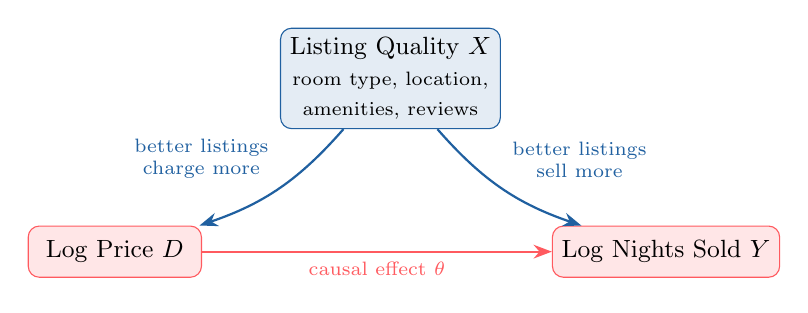
\begin{tikzpicture}[node distance=1.8cm and 2.8cm]
\node[tblue] (X) at (3.5, 2.2) {Listing Quality $X$\\{\scriptsize room type, location,}\\{\scriptsize amenities, reviews}};
\node[tred]  (D) at (0, 0)     {Log Price $D$};
\node[tred]  (Y) at (7, 0)     {Log Nights Sold $Y$};

\draw[tarrow, noteblue, bend left=15]
    (X) to node[above left, font=\scriptsize, align=center]{better listings\\charge more} (D);
\draw[tarrow, noteblue, bend right=15]
    (X) to node[above right, font=\scriptsize, align=center]{better listings\\sell more} (Y);
\draw[tarrow, thick, abnbred]
    (D) -- node[below, font=\scriptsize]{causal effect $\theta$} (Y);
\end{tikzpicture}
\end{center}

\pause

$X$ is a \textbf{confounder}: it opens the backdoor path $D \leftarrow X \rightarrow Y$. Conditioning on $X$ blocks this path. Among listings with identical $X$, remaining price variation is as-if random.

\bigskip

\textbf{In the running example:} within type $A$, the slope of $Y$ on $D$ is $-1$ (the true $\theta$). Within type $B$ likewise. Comparing across types is what caused the $+1.06$ bias.

\end{frame}

% ====================================================================
\begin{frame}{Good Controls and Bad Controls}
\begin{figure}
    \centering
    \includegraphics[width=.95\linewidth]{fig/controls.png}
    % \caption{Enter Caption}
    \label{fig:controls}
\end{figure}
\end{frame}


\begin{frame}{Good Controls and Bad Controls}

Not every variable belongs in $X$. Including the wrong ones \textbf{introduces new bias}.

\bigskip

\begin{center}
\begin{tabular}{lcl}
\toprule
\textbf{Type} & \textbf{Include?} & \textbf{Why} \\
\midrule
Confounder  & \textcolor{noteblue}{Yes} & Closes backdoor path \\
Mediator    & \textcolor{warnred}{No}  & Blocks part of the causal effect \\
Collider    & \textcolor{warnred}{No}  & Opens a new spurious path \\
\bottomrule
\end{tabular}
\end{center}

\bigskip
\pause

\textbf{Confounders} (room type, neighbourhood, amenities): affect both $D$ and $Y$. Include them.

\bigskip

\textbf{Mediators} (search rank): price $\to$ rank $\to$ bookings. Controlling for rank blocks the indirect effect and biases $\hat{\theta}$ toward zero.

\bigskip

\textbf{Colliders} (number of reviews): affected by both nights sold and prices. Conditioning on it opens a spurious path and biases $\hat{\theta}$.

\end{frame}
% ====================================================================
\begin{frame}{Is Unconfoundedness Credible?}

Once good controls are selected, unconfoundedness says: among listings with the same $X$, remaining price variation is exogenous. This is \textbf{substantive and untestable.}

\begin{center}
\small
\begin{tabular}{lll}
\toprule
\textbf{Quality signal} & \textbf{Observed?} & \textbf{Status} \\
\midrule
Room type, neighbourhood    & \textcolor{noteblue}{Yes} & Controlled for \\
Amenity count, review score & \textcolor{noteblue}{Yes} & Controlled for \\
Host tenure                 & \textcolor{noteblue}{Yes} & Controlled for \\
Photo quality, decor        & \textcolor{warnred}{No}   & Residual confounding \\
Host responsiveness         & \textcolor{warnred}{No}   & Residual confounding \\
\bottomrule
\end{tabular}
\end{center}

\pause

\textbf{The challenge:} we can never be sure we have included all relevant confounders. We don't know what we don't know (hidden confounders).

\bigskip

\textbf{Professional standard:} state the assumption explicitly, defend it with domain knowledge, select controls using the DAG, and report sensitivity analysis.

\end{frame}


% ====================================================================
\begin{frame}{Key Takeaways}

\begin{enumerate}
    \item \textbf{Isoelastic demand motivates the log-log regression and the target $\theta$.} $\theta$ is the sufficient statistic for pricing. $g(X)$ is a nuisance that confounds naive estimation.

    \pause\bigskip

    \item \textbf{Three assumptions identify causal effects.} Consistency/SUTVA, unconfoundedness, and overlap identify the ADRF (Theorem 1) as well as its slope (Theorem 2).

    \pause\bigskip

    \item \textbf{OLS and Lasso each have limitations.} OLS with linear controls cannot capture nonlinear $g(X)$. Lasso handles the dimensionality but introduces regularization bias on $\hat{\theta}$ and invalid post-selection inference.
    
    \pause\bigskip

    \item \textbf{The DAG decides which controls to include.} Confounders in, mediators and colliders out. The credibility of unconfoundedness depends on how much residual confounding remains; however, this is more of art than science. 

\end{enumerate}

\end{frame}

\end{document}